%% The '3p' and 'times' class options of elsarticle are used for Elsevier CRC
%% Add the 'procedia' option to approximate to the Word template
%\documentclass[3p,times,procedia]{elsarticle}
\documentclass[3p,times]{elsarticle}

%% The `ecrc' package must be called to make the CRC functionality available
\usepackage{ecrc}
\usepackage{color,soul}
\usepackage{multirow}
\usepackage{booktabs}
\graphicspath{{images/}}

\usepackage{lscape}


\volume{00}
\firstpage{1}
\journalname{Forest ecology and management}
\runauth{Gilles A. et al.}

%% Give the abbreviation of the Journal. %% A user-supplied logo with the name <\jid>logo.pdf will be inserted if present.
\jid{feam}
\jnltitlelogo{Forest ecology and management}
\CopyrightLine{2022}{Published by Elsevier Ltd.}

\usepackage{amssymb}
\usepackage{lineno}

\usepackage{hyperref}
\usepackage{subfig}
\usepackage[export]{adjustbox}

% if you have landscape tables
%\usepackage[figuresright]{rotating}
% add words to TeX's hyphenation exception list
%\hyphenation{author another created financial paper re-commend-ed Post-Script}

\begin{document}

\begin{frontmatter}

%% Title, authors and addresses

%% use the tnoteref command within \title for footnotes;
%% use the tnotetext command for the associated footnote;
%% use the fnref command within \author or \address for footnotes;
%% use the fntext command for the associated footnote;
%% use the corref command within \author for corresponding author footnotes;
%% use the cortext command for the associated footnote;
%% use the ead command for the email address,
%% and the form \ead[url] for the home page:
%%
%% \title{Title\tnoteref{label1}}
%% \tnotetext[label1]{}
%% \author[label1,label2]{<author name>}
\author[label2]{Gilles Arthur}
\ead{tonemail}
\author[label2]{Lisein Jonathan}
%\ead{liseinjon@hotmail.com}
\author[label2]{Claessens Hugues}

%% \ead[url]{home page}
\fntext[label2]{Liège University - Faculty of Gembloux Agro-Bio Tech - unit of forest ressources managment}
%\fntext[label1]{Forêt.Nature asbl}
%\cortext[cor1]{}
%% \address{Address\fnref{label3}}
%% \fntext[label3]{}

\dochead{Original research papers}
%% Use \dochead if there is an article header, e.g. \dochead{Short communication}
%% \dochead can also be used to include a conference title, if directed by the editors
%% e.g. \dochead{17th International Conference on Dynamical Processes in Excited States of Solids}

%pdftotext 2021-phytoSpy.pdf - | tr -d '.' | wc -w pour le nombre de mot

\title{Ips Typographus behaviour show notable differences between Belgium and north France : a remote sensing analysis of 2016-2021 spruce dieback}

\begin{abstract}

\end{abstract}

\begin{keyword}
% nutrient regime \sep moisture regime
\end{keyword}

\end{frontmatter}

\linenumbers

\pagebreak
\section{Introduction}

\begin{itemize}
	\item Aire de répartition de l'épicéa
	\item Scolyte description générale, plus précision typographe chalcographe
	\item Evolution des dégats lié au scolyte dans le monde
	\item Début de la crise en Wallonie + Vosges en 2018
	\item Objectif de l'article: caractérisation des attaque de scolytes en Wallonie et dans les Vosges selon deux variables environnementales +paramètres macro 
\end{itemize}

\section{Matériel et méthode}

\subsection{Description zone de la Zone d'étude}

\begin{itemize}
	\item Description zone d'étude générale + tuile S2 traitées (figure: \ref{fig:rep_vosg}) 
	\item Description générale de la forêt wallonne 
	\item Description de la pessière wallonne (figure: \ref{fig:rep_wal})
	\item Description générale de la foret vosgienne 
	\item Description de la pessière vosgienne (figure: \ref{fig:rep_vosg})
	\item Comparaison Température et précipitation vosges et Wallonie entre moyenne trentenaire et données pour l'année 2018 (figure \ref{fig:diagOT})
	
\end{itemize}



\subsection{Données de MNT et de Sous-secteurs Radiatif}

\begin{itemize}
	\item Provenance des données de MNT
	\item Méthodologie de calcul des sous-secteur radiatif.
\end{itemize}


\subsection{Mapping of spruce dieback and mortality by analysis of sentinel-2 time-serie}
\citep{bolyn_forest_2018}

\citep{grabska_forest_2019,ma_tree_2021,abdullah_sentinel-2_2019}

% mask ep
% méthode de détection
\begin{figure}
	\centering
	\includegraphics[width=\textwidth]{fctHarmo-page001.png}
	\caption{Modelisation of seasonal variation of CRSWIR vegetation indice accros vegetetion period for a spuce stand.}
	\label{fig:harmo}
\end{figure}

\subsection{Analyse stat}
\begin{itemize}
	\item test de student 
\end{itemize}

\section{résultats}

\subsection{ Altitude vs probabilité de présence de scolyte}



\begin{itemize}
	\item Description figure \ref{fig:sco_alti}
	\item Wallonie: Diminution de la probabilité de présence de scolyte avec l'augmentation de l'altitude 
	\item Vosges pas de relation clair avec l'altitude. Cependant, les classes d'altitude 2, 11 et 12 semblent + touchées que les autres classes d'altitude
	
	\item Wallonie + Vosges: Augmentation de la probabilité de présence de scolyte avec le temps quelque soit la classe d'altitude.
\end{itemize}



\subsection{Sous-secteur radiatif vs probabilité de présence de scolyte}


\begin{itemize}
	\item Description figure \ref{fig:ss_wall} 
	\item Wallonie: Différences significative entre les différents sous secteurs. Les sous secteur froid sont  plus touchés que les sous secteur chaud et les plateaux. Les plateaux sont moins touché en Wallonie.
	\item Vosges: pas de différence significative entre les sous secteurs ( \ref{fig:ss_vosg})
	
\end{itemize}

%sous-secteur
%graphe + descruipton


\section{Discussion}

\subsection{Différence entre Vosges et Wallonie}
\begin{itemize}
	\item Différence climat (Climat semicontinental/montagnard vs climat tempéré océanique)
	\item Différence sylvicole ( Wallonie futaie régulière exploitable vs Vosges peuplement + mélangé et moins exploitable en haute altitude)
	\item Sommet des vosges epicéas endémiques vs épicéas en plantations (résilience peuplement )
	
\end{itemize}

\subsection{Facteur déterminant l'attaque par l'épicéa ou le scolyte}

\begin{itemize}
	\item Discussion généralisation de modèle scolyte/ dépérissement des épicéas
	\item est ce la Biologie du scolyte/ ou le stress de l'épicéa qui conditionne le dépérissement massif ?
	
\end{itemize}

\section{Conclusion}

Dépérissement différents pour les Vosges et la Wallonie.

\section{Figure}

\begin{figure} [htbp] 
	\centering
	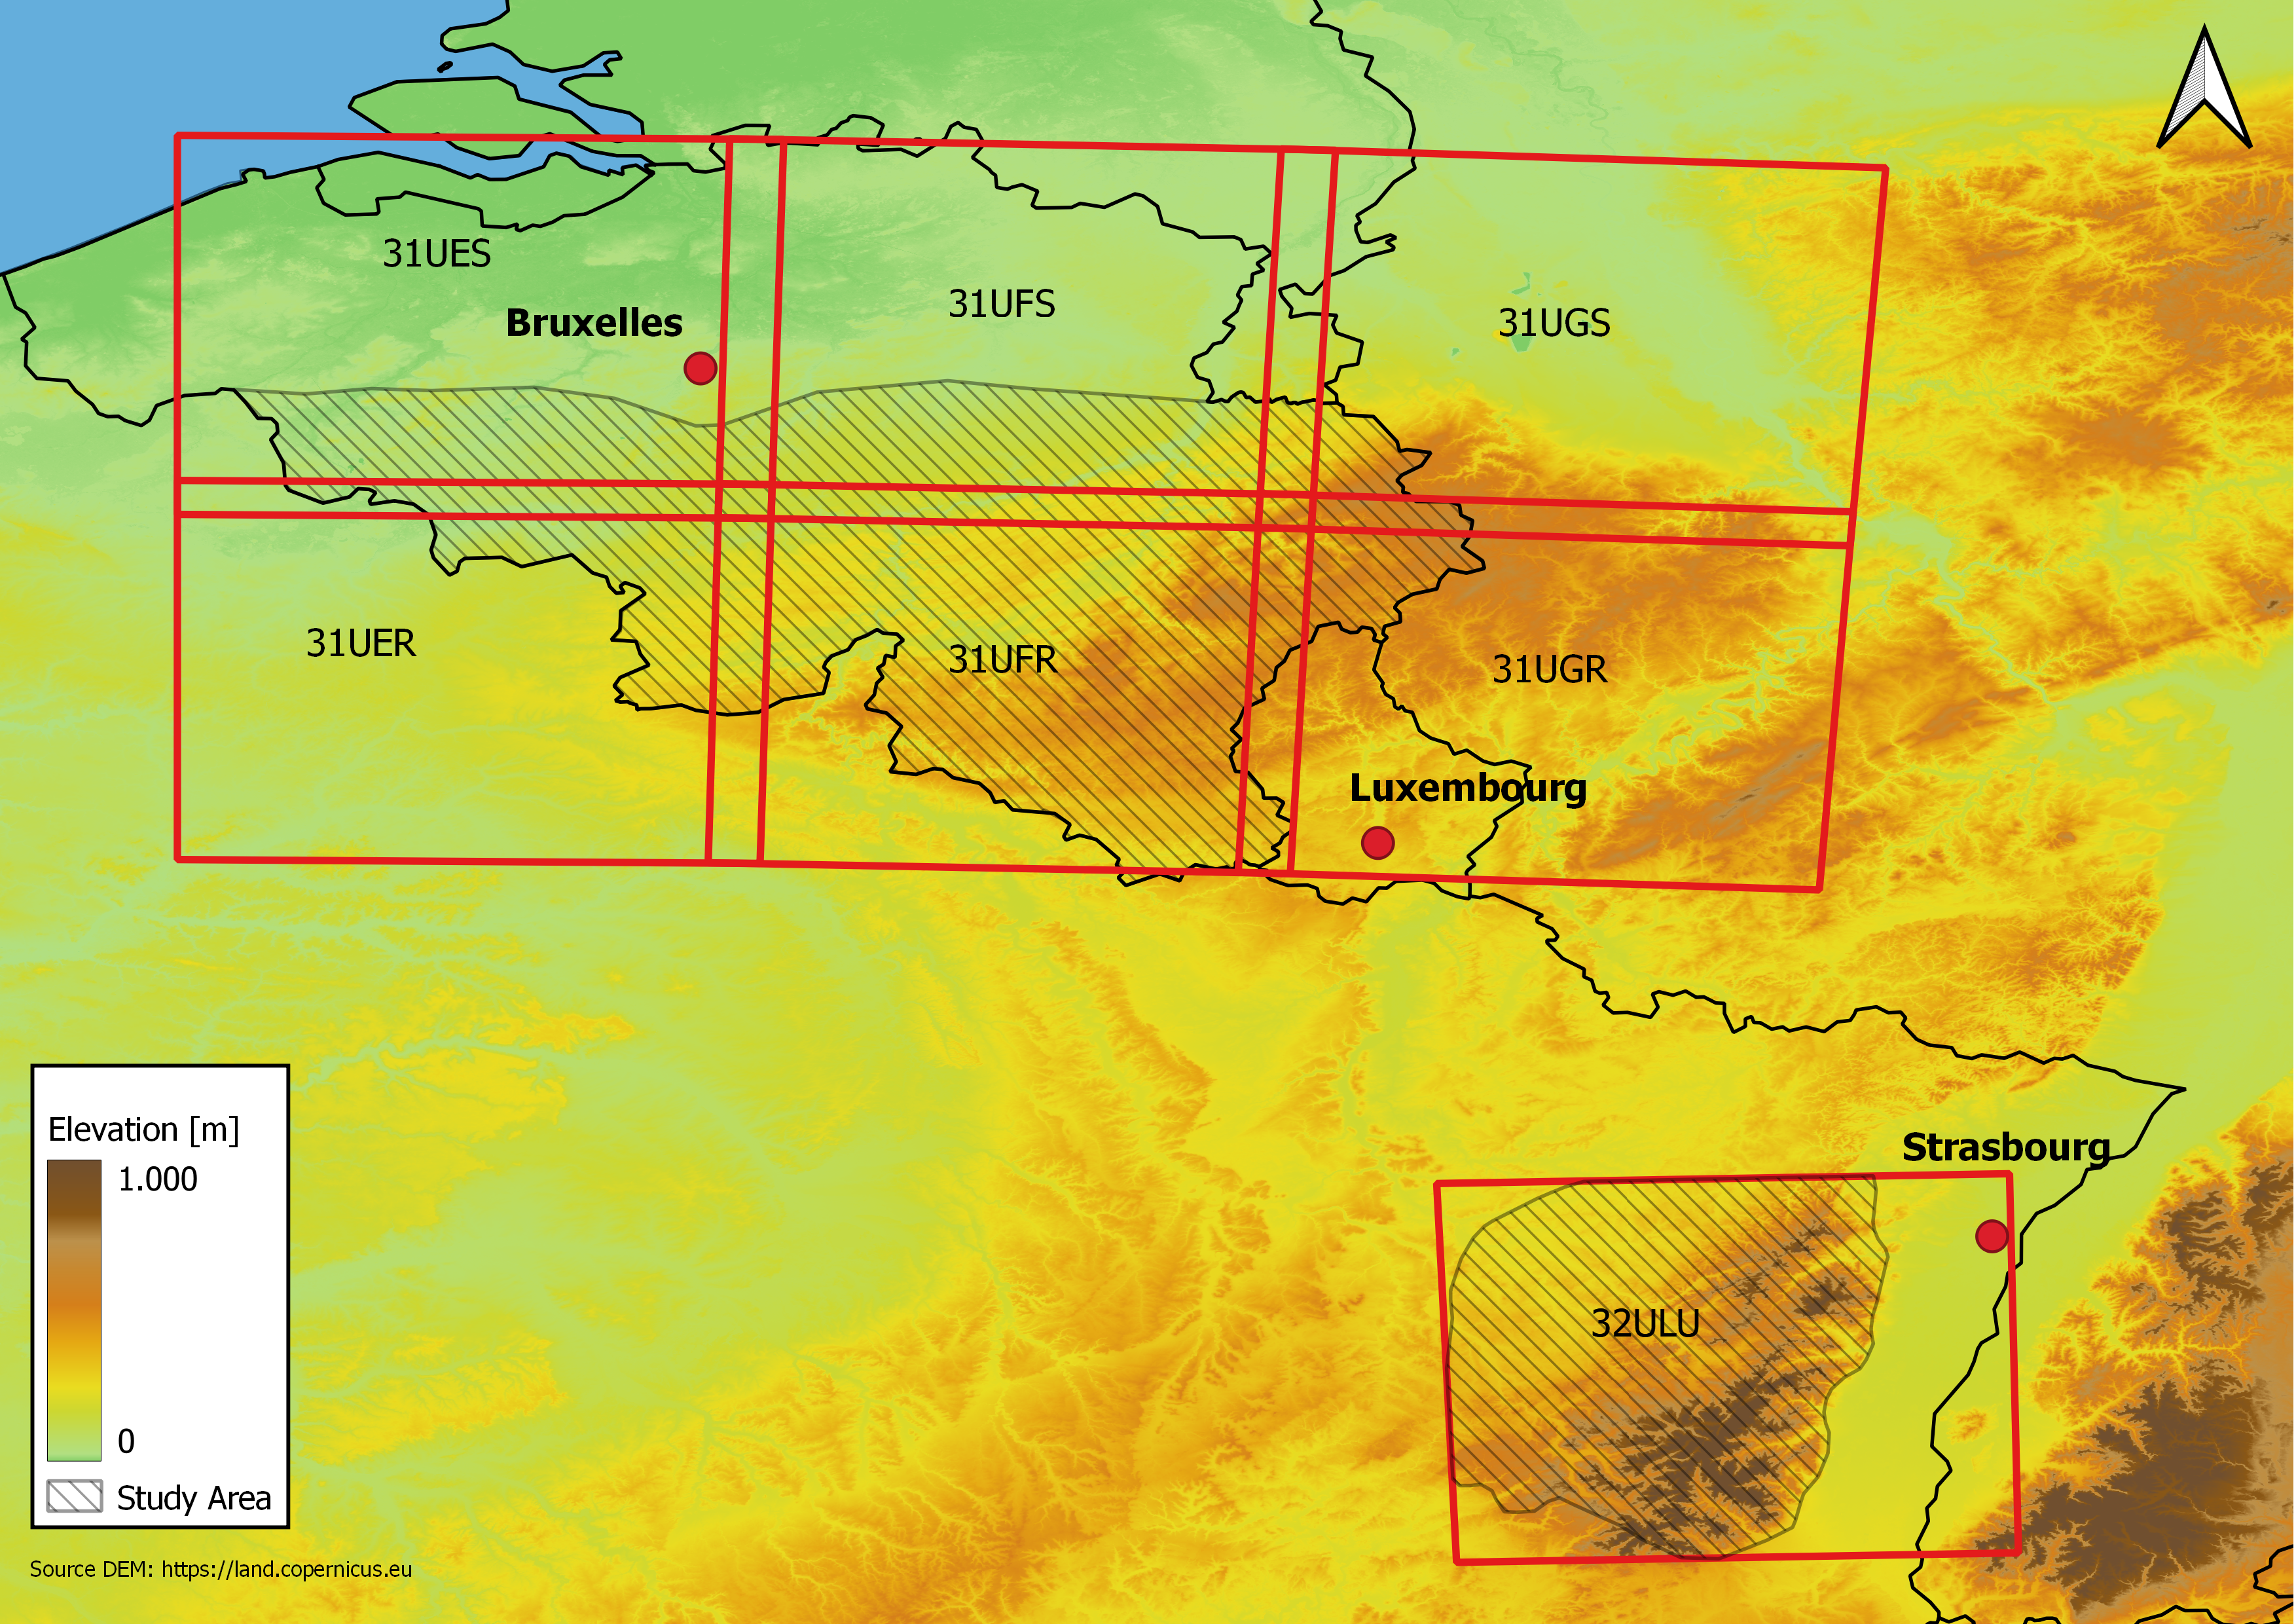
\includegraphics[width=1\textwidth]{waql_2.png}
	\caption{Zones d'études avec le MNT (XXX) et les tuiles du satellite Sentinelle 2 employées(XXX légende carré rouge).}
	\label{fig:situ}
\end{figure}
\begin{figure}[htbp]
	\begin{minipage}[b]{1 \linewidth}
		\centering
		\includegraphics[width=1\textwidth]{elevation_spruce_stand_wall.png}
		\caption{Répartition de la pessière wallonne en fonction de l'altitude en 2018.}
		\label{fig:rep_wal}
		%\caption sert à insérer une légende
	\end{minipage}\hfill
	\vspace{1cm}
	\begin{minipage}[b]{1 \linewidth}
		\centering
		\includegraphics[width=1\textwidth]{elevation_spruce_stand_vosge.png}
		\caption{Répartition de la pessière vosgienne en fonction de l'altitude en 2018.}
		\label{fig:rep_vosg}
	\end{minipage}
\end{figure}

\begin{figure} [htbp] 
	\centering
	\includegraphics[width=1\textwidth]{diagrammeOT-page001.png}
	\caption{Walter and Lieth climatic diagram comparison for Ardenne (up) and Vosges (down). Left diagram show the average recent climate, and rigth one illustrates the year of 2018.}
	\label{fig:diagOT}
\end{figure}


\begin{figure} [htbp] 
		\centering
		\includegraphics[width=1\textwidth]{Wall_vs_vosges.png}
		\caption{Probabilité de présence de scolyte en fonction de l'altitude pour la Wallonie et les Vosges}
		\label{fig:sco_alti}
\end{figure}
	

\begin{figure}[htbp]
	\begin{minipage}[b]{1 \linewidth}
		\centering
	%	\includegraphics[width=1\textwidth]{evol_ss_wal.png}
		\caption{Évolution de la crise du typographe en région wallonne en fonction des sous-secteurs.}
		\label{fig:ss_wall}
		%\caption sert à insérer une légende
	\end{minipage}\hfill
	\vspace{1cm}
	\begin{minipage}[b]{1 \linewidth}
		\centering
		\includegraphics[width=1\textwidth]{evol_ss_vosges.png}
		\caption{Évolution de la crise du typographe dans les Vosges en fonction des sous-secteurs .}
		\label{fig:ss_vosg}
	\end{minipage}
\end{figure}

\section{Acknowledgements}

This research has been funded thanks to the \textit{RegioWood II} project.

\bibliographystyle{elsarticle-num}
%\bibliographystyle{elsarticle-harv}\biboptions{authoryear}
\bibliography{Scolyte.bib}
\end{document}